\section{What is Open-Source?}

\begin{frame}[fragile]{Definition of Open Source}
%\addcontentsline{toc}{subsection}{Definition of Open Source}
\makebox[\textwidth][c]{
\begin{figure}
    \centering
    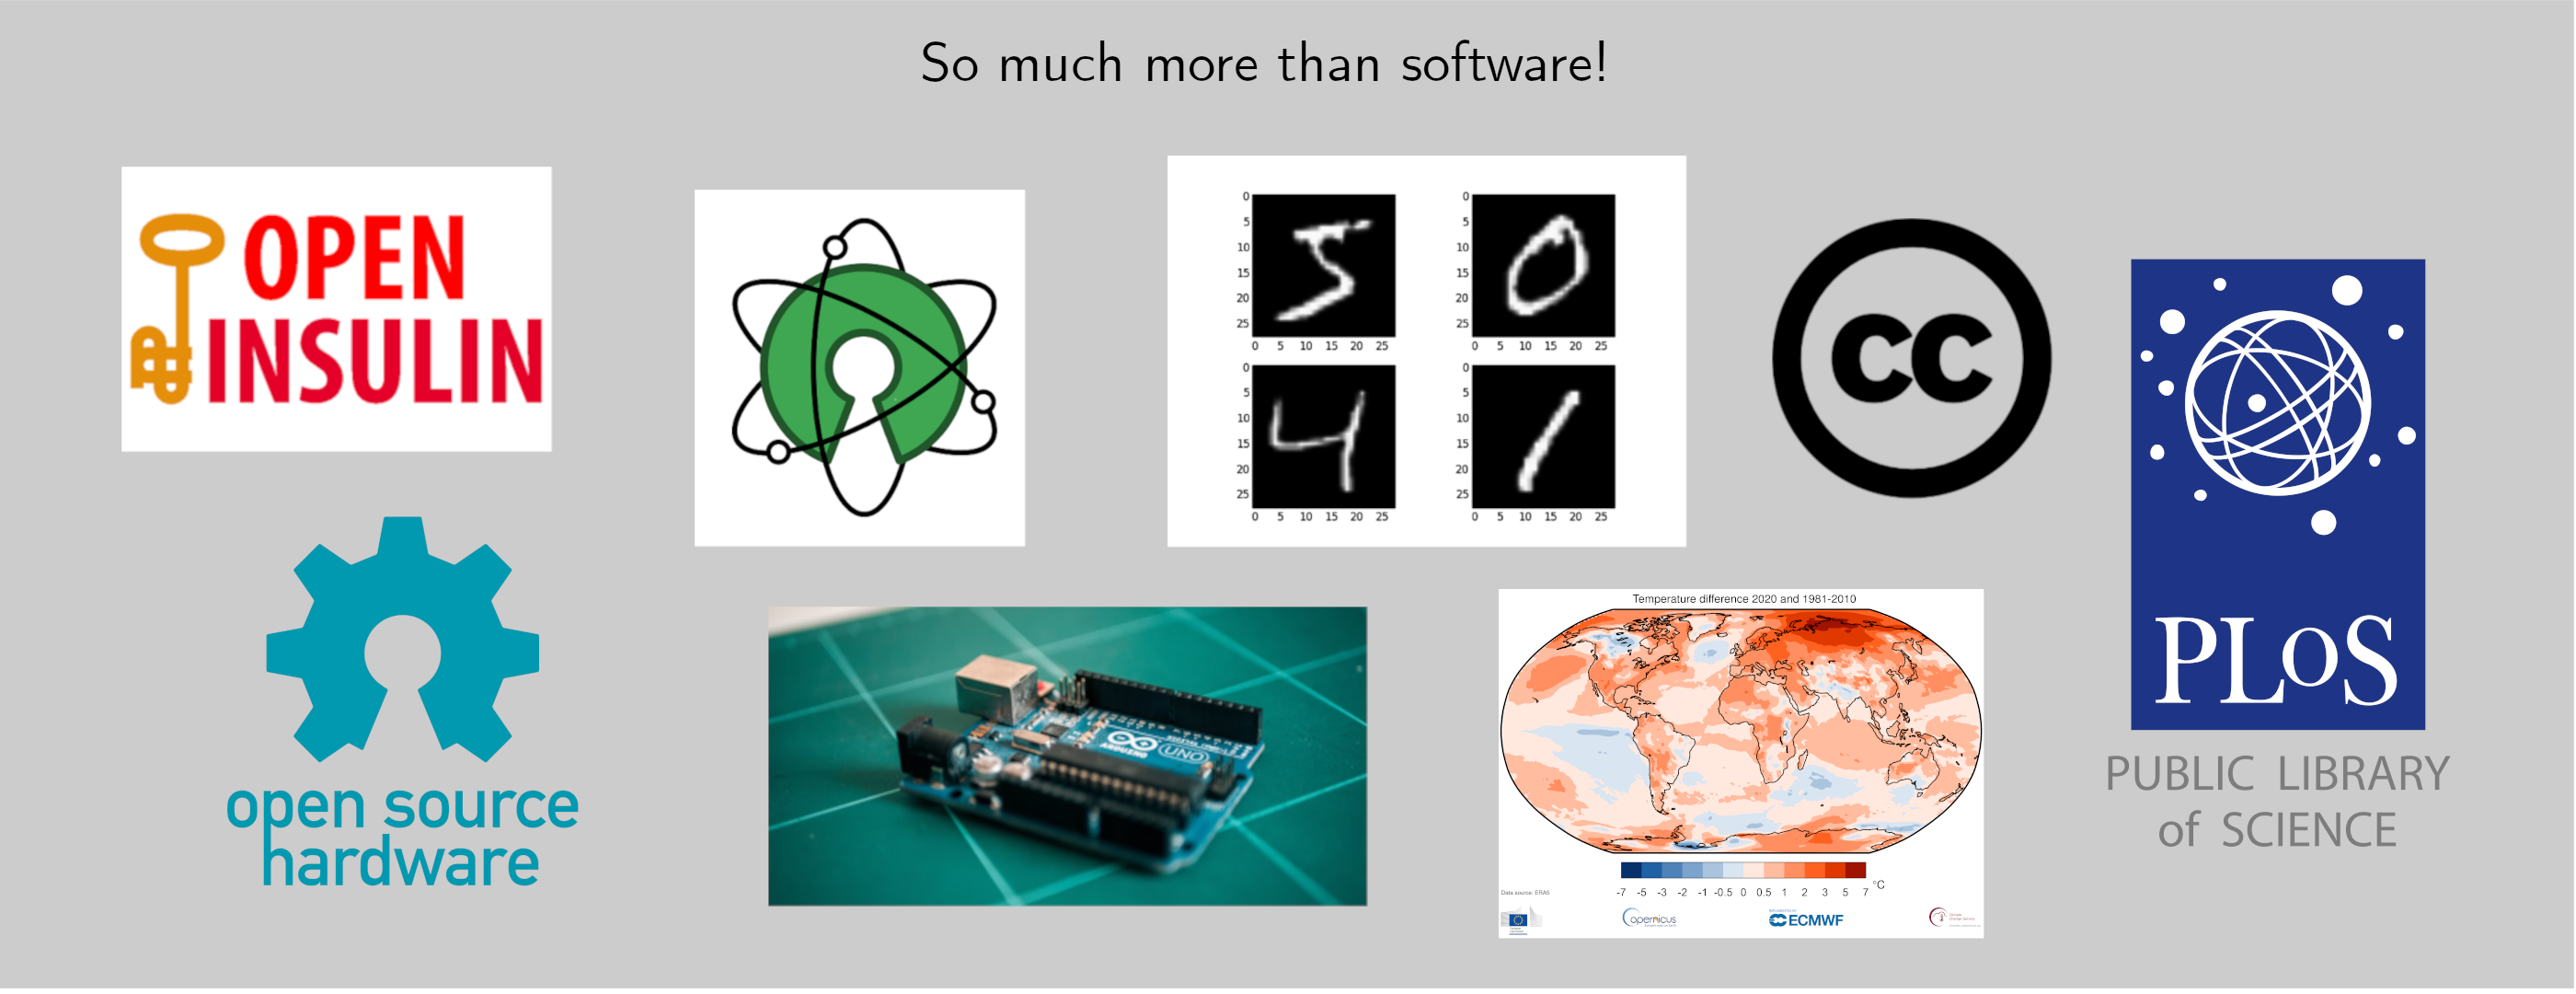
\includegraphics[width=1.1\linewidth]{assets/Untitled.png}
\end{figure}}
\end{frame}

\automateframe{Key Characteristics}{
\begin{itemize}
    \item Transparency
    \item Collaboration
    \item Community-driven Development
    \item Innovation and Iteration
    \item Freedom to Use and Modify
    \item Licensing
\end{itemize}
}

\begin{frame}[fragile]{Licensing}
\makebox[\textwidth][c]{
\begin{figure}
    \centering
    
\includegraphics[width=1.1\linewidth]{assets/Licenses.png}
\end{figure}
}
\end{frame}